\documentclass[tikz,border=5pt]{standalone}
% Scale s = 0.009988 cm/px, origin at ink-bbox centre (457.5, 346.5), y flipped
\begin{document}
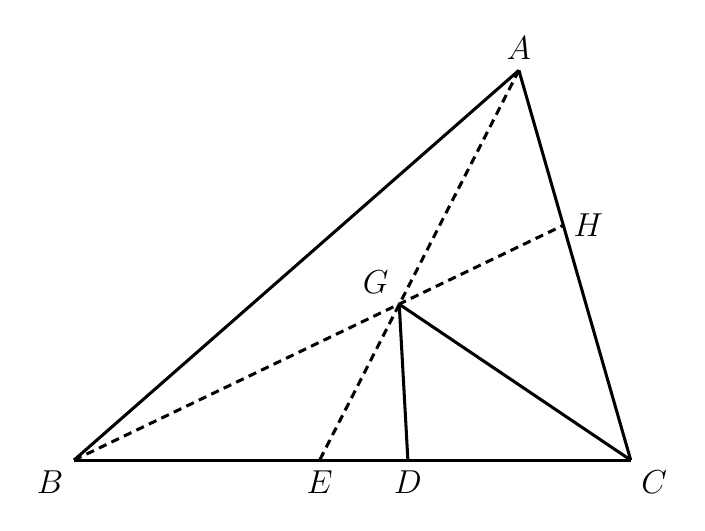
\begin{tikzpicture}[line width=1.1pt, line join=round]

% Named coordinates (converted from pixels)
\coordinate (A) at (2.11,2.48);
\coordinate (B) at (-3.54,-2.47);
\coordinate (C) at (3.53,-2.47);
\coordinate (D) at (0.70,-2.47);
\coordinate (E) at (-0.42,-2.47);
\coordinate (G) at (0.59,-0.49);
\coordinate (H) at (2.67,0.51);

% Solid triangle and cevian segments
\draw (A) -- (B);
\draw (A) -- (C);
\draw (B) -- (C);
\draw (G) -- (C);
\draw (G) -- (D);

% Dashed cevians through G
\draw[dash pattern=on 3pt off 2pt] (A) -- (E);
\draw[dash pattern=on 3pt off 2pt] (B) -- (H);

% Labels: explicit 12/14 pt font as requested (anchors unchanged)
\node[font=\fontsize{12}{14}\selectfont, above] at (A) {$A$};
\node[font=\fontsize{12}{14}\selectfont, below left] at (B) {$B$};
\node[font=\fontsize{12}{14}\selectfont, below right] at (C) {$C$};
\node[font=\fontsize{12}{14}\selectfont, below] at (D) {$D$};
\node[font=\fontsize{12}{14}\selectfont, below] at (E) {$E$};
\node[font=\fontsize{12}{14}\selectfont, right] at (H) {$H$};
\node[font=\fontsize{12}{14}\selectfont, above left] at (G) {$G$};

\end{tikzpicture}
\end{document}